\newpage
\appendix

\section{Appendix}

\subsection{Low fidelity prototypes} \label{app_low_fidelity}

\begin{figure}[!htb]
    \centering
    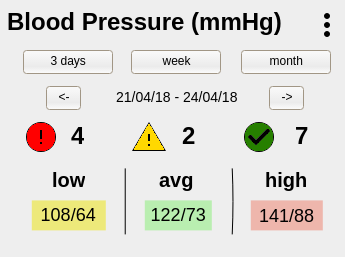
\includegraphics[width=0.45\textwidth]{chapters/3_design/mockups/bp_small}
    \caption{Small blood pressure module}\label{fig:bp_small}
\end{figure}

\begin{figure}[!htb]
    \centering
    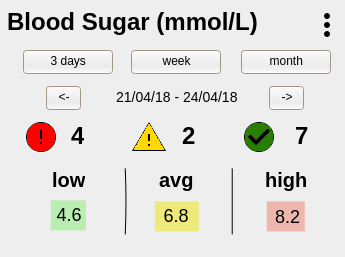
\includegraphics[width=0.45\textwidth]{chapters/3_design/mockups/bs_small}
    \caption{Small blood sugar module}\label{fig:bs_small}
\end{figure}

\begin{figure}[!htb]
    \centering
    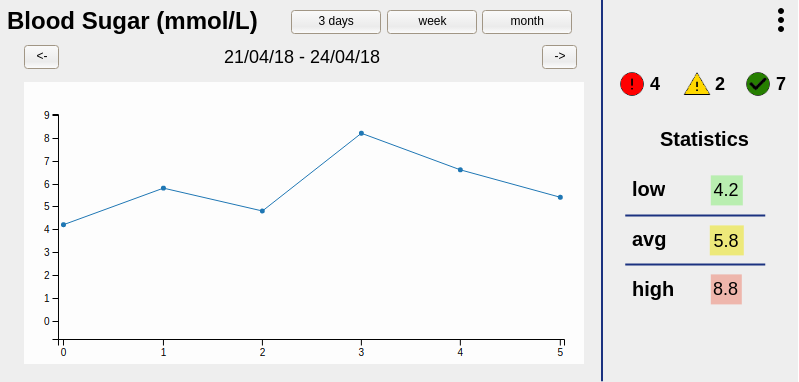
\includegraphics[width=0.75\textwidth]{chapters/3_design/mockups/bs_large}
    \caption{Large blood sugar module}\label{fig:bs_large}
\end{figure}

\begin{figure}[!htb]
    \centering
    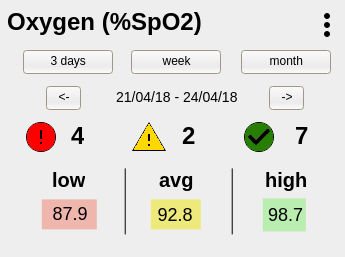
\includegraphics[width=0.45\textwidth]{chapters/3_design/mockups/oxygen_small}
    \caption{Small oxygen module}\label{fig:oxygen_small}
\end{figure}

\begin{figure}[!htb]
    \centering
    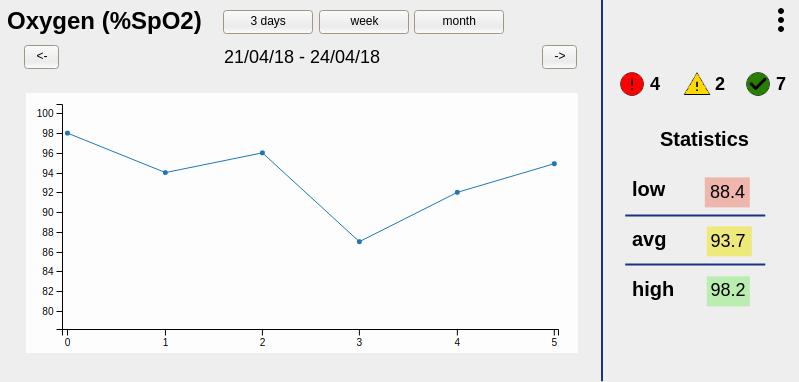
\includegraphics[width=0.75\textwidth]{chapters/3_design/mockups/oxygen_large}
    \caption{Large oxygen module}\label{fig:oxygen_large}
\end{figure}

\clearpage
\subsection{REST API documentation} \label{app_rest_api}

    \subsubsection{User}

        The user module was created to show basic information and does not offer much functionality.

        \paragraph{Create user} Creates a new user in the database.
        \begin{itemize}
            \item \textbf{URL}: /user
            \item \textbf{Method}: \texttt{POST}
            \item \textbf{Data Params}: \begin{verbatim}
    {
        "firstName": "John",
        "lastName": "Doe",
        "birth": "1998-09-15T15:53:00",
        "gender": "M",
        "bloodType": "O+",
        "height": "1.77m",
        "address": "Agoralaan, 3590 Diepenbeek",
        "phone": "0123/456789"
    }
            \end{verbatim}
        \end{itemize}

        \paragraph{Get user} Get the information of a user according to the supplied id.
        \begin{itemize}
            \item \textbf{URL}: /user/:id
            \item \textbf{Method}: \texttt{GET}
            \item \textbf{URL Params}: \texttt{id=[string]}
            \item \textbf{Response}: \begin{verbatim}
    {
        "_id": "5b5c65e3ad30264506380dd1",
        "firstName": "John",
        "lastName": "Doe",
        "birth": "2008-09-15T15:53:00",
        "gender": "M","bloodType": "O+",
        "height": "1.77m",
        "address": "Agoralaan, 3590 Diepenbeek",
        "phone": "0123/456789"
    }
            \end{verbatim}
        \end{itemize}

    \subsubsection{Blood pressure}

        \paragraph{Get blood pressure values for large module} Get blood pressure values within given period.
        \begin{itemize}
            \item \textbf{URL}: /bp/:start\&:end
            \item \textbf{Method}: \texttt{GET}
            \item \textbf{URL Params}: \texttt{start=[integer], end=[integer]}
            \item \textbf{Response}: \begin{verbatim}
    {
        "thresholds": Object,
        "values": Array,
        "avgLine": Array // contains info to draw 
    }                    // average lines on chart
            \end{verbatim}
        \end{itemize}

        \paragraph{Get blood pressure statistics for small module} Get blood pressure statistics within given period.
        \begin{itemize}
            \item \textbf{URL}: /bp/small/:start\&:end
            \item \textbf{Method}: \texttt{GET}
            \item \textbf{URL Params}: \texttt{start=[integer], end=[integer]}
            \item \textbf{Response}: \begin{verbatim}
    {
        "low": "110/68",
        "high": "131/88",
        "avg": "119.7/78.0",
        "dangerVals": 1,
        "warningVals": 1,
        "okVals": 1,
        "lowCol": "yellow",
        "avgCol": "green",
        "highCol": "red",
        "thresholds": Object
    }
            \end{verbatim}
        \end{itemize}

        \paragraph{Create blood pressure entry} Creates a new blood pressure entry in the database.
        \begin{itemize}
            \item \textbf{URL}: /bp
            \item \textbf{Method}: \texttt{POST}
            \item \textbf{Data Params}: \begin{verbatim}
    {
        "systolic": "118",
        "diastolic": "78",
        "date": "2018-07-30T16:39:12Z"
    }   
            \end{verbatim}
        \end{itemize}

        \paragraph{Create thresholds} Creates default thresholds for user.
        \begin{itemize}
            \item \textbf{URL}: /bp/threshold
            \item \textbf{Method}: \texttt{POST}
        \end{itemize}

        \paragraph{Update thresholds} Updates thresholds for user.
        \begin{itemize}
            \item \textbf{URL}: /bp/threshold
            \item \textbf{Method}: \texttt{PATCH}
            \item \textbf{Data Params}: \begin{verbatim}
    {
        "warningLess": "40",
        "warningHigher": "41",
        "dangerLess": "42",
        "dangerHigher": "43"
    }  
            \end{verbatim}
        \end{itemize}

        \paragraph{Get threshold values} Get threshold values for user.
        \begin{itemize}
            \item \textbf{URL}: /bp/threshold
            \item \textbf{Method}: \texttt{GET}
            \item \textbf{Response}: \begin{verbatim}
    {
        "_id": "5b684666c0e0e", // id from main route
        "warningLess": 75,
        "warningHigher": 120,
        "dangerLess": 40,
        "dangerHigher": 130
    }
            \end{verbatim}
        \end{itemize}

    \subsubsection{Blood sugar}

        \paragraph{Get blood sugar values for large module} Get blood sugar values within given period.
        \begin{itemize}
            \item \textbf{URL}: /bs/:start\&:end
            \item \textbf{Method}: \texttt{GET}
            \item \textbf{URL Params}: \texttt{start=[integer], end=[integer]}
            \item \textbf{Response}: \begin{verbatim}
    {
        "thresholds": Object,
        "values": Array,
        "avgLine": Array // contains info to draw 
    }                    // average lines on chart
            \end{verbatim}
        \end{itemize}

        \paragraph{Get blood sugar statistics for small module} Get blood sugar statistics within given period.
        \begin{itemize}
            \item \textbf{URL}: /bs/small/:start\&:end
            \item \textbf{Method}: \texttt{GET}
            \item \textbf{URL Params}: \texttt{start=[integer], end=[integer]}
            \item \textbf{Response}: \begin{verbatim}
    {
        "low": "3.8",
        "high": "6.7",
        "avg": "5.2",
        "dangerVals": 0,
        "warningVals": 2,
        "okVals": 1,
        "lowCol": "yellow",
        "avgCol": "green",
        "highCol": "yellow",
        "thresholds": Object
    }
            \end{verbatim}
        \end{itemize}

        \paragraph{Create blood sugar entry} Creates a new blood sugar entry in the database.
        \begin{itemize}
            \item \textbf{URL}: /bs
            \item \textbf{Method}: \texttt{POST}
            \item \textbf{Data Params}: \begin{verbatim}
    {
        "value": "6.7",
        "date": "2018-07-30T16:39:12Z"
    }   
            \end{verbatim}
        \end{itemize}

        \paragraph{Create thresholds} Creates default thresholds for user.
        \begin{itemize}
            \item \textbf{URL}: /bs/threshold
            \item \textbf{Method}: \texttt{POST}
        \end{itemize}

        \paragraph{Update thresholds} Updates thresholds for user.
        \begin{itemize}
            \item \textbf{URL}: /bs/threshold
            \item \textbf{Method}: \texttt{PATCH}
            \item \textbf{Data Params}: \begin{verbatim}
    {
        "warningLess": "4",
        "warningHigher": "6",
        "dangerLess": "3",
        "dangerHigher": "8"
    }  
            \end{verbatim}
        \end{itemize}

        \paragraph{Get threshold values} Get threshold values for user.
        \begin{itemize}
            \item \textbf{URL}: /bs/threshold
            \item \textbf{Method}: \texttt{GET}
            \item \textbf{Response}: \begin{verbatim}
    {
        "_id": "5b684666c0e0e", // id from main route
        "warningLess": 4,
        "warningHigher": 6,
        "dangerLess": 3,
        "dangerHigher": 8
    }
            \end{verbatim}
        \end{itemize}

    \subsubsection{Heart rate}

        \paragraph{Get heart rate values for large module} Get heart rate values within given period.
        \begin{itemize}
            \item \textbf{URL}: /heart/:start\&:end
            \item \textbf{Method}: \texttt{GET}
            \item \textbf{URL Params}: \texttt{start=[integer], end=[integer]}
            \item \textbf{Response}: \begin{verbatim}
    {
        "thresholds": Object,
        "values": Array,
        "avgLine": Array // contains info to draw 
    }                    // average lines on chart
            \end{verbatim}
        \end{itemize}

        \paragraph{Get heart rate statistics for small module} Get heart rate statistics within given period.
        \begin{itemize}
            \item \textbf{URL}: /heart/small/:start\&:end
            \item \textbf{Method}: \texttt{GET}
            \item \textbf{URL Params}: \texttt{start=[integer], end=[integer]}
            \item \textbf{Response}: \begin{verbatim}
    {
        "low": "38",
        "high": "78",
        "avg": "56.0",
        "dangerVals": 0,
        "warningVals": 1,
        "okVals": 2,
        "lowCol": "yellow",
        "avgCol": "green",
        "highCol": "green",
        "thresholds": Object
    }
            \end{verbatim}
        \end{itemize}

        \paragraph{Create heart rate entry} Creates a new heart rate entry in the database.
        \begin{itemize}
            \item \textbf{URL}: /heart
            \item \textbf{Method}: \texttt{POST}
            \item \textbf{Data Params}: \begin{verbatim}
    {
        "value": "62",
        "date": "2018-07-30T16:39:12Z"
    }   
            \end{verbatim}
        \end{itemize}

        \paragraph{Create thresholds} Creates default thresholds for user.
        \begin{itemize}
            \item \textbf{URL}: /heart/threshold
            \item \textbf{Method}: \texttt{POST}
        \end{itemize}

        \paragraph{Update thresholds} Updates thresholds for user.
        \begin{itemize}
            \item \textbf{URL}: /heart/threshold
            \item \textbf{Method}: \texttt{PATCH}
            \item \textbf{Data Params}: \begin{verbatim}
    {
        "warningLess": "40",
        "warningHigher": "80",
        "dangerLess": "30",
        "dangerHigher": "95"
    }  
            \end{verbatim}
        \end{itemize}

        \paragraph{Get threshold values} Get threshold values for user.
        \begin{itemize}
            \item \textbf{URL}: /heart/threshold
            \item \textbf{Method}: \texttt{GET}
            \item \textbf{Response}: \begin{verbatim}
    {
        "_id": "5b684666c0e0e", // id from main route
        "warningLess": 40,
        "warningHigher": 80,
        "dangerLess": 30,
        "dangerHigher": 95
    }
            \end{verbatim}
        \end{itemize}

    \subsubsection{Medication}

        \paragraph{Get medication adherence for large module} Get medication adherence within given period.
        \begin{itemize}
            \item \textbf{URL}: /medication/:start\&:end
            \item \textbf{Method}: \texttt{GET}
            \item \textbf{URL Params}: \texttt{start=[integer], end=[integer]}
            \item \textbf{Response}: \begin{verbatim}
    {
        "thresholds": Object,
        "values": Array,
        "dates": Array, // dates for each value
        "xsDates": Array, // array to pair each medicine
                          // to line on chart
        "indivStrings": Array // contains adherence 
    }                         // fractures for tooltips
            \end{verbatim}
        \end{itemize}

        \paragraph{Get medication adherence averages for small module} Get medication adherence averages within given period.
        \begin{itemize}
            \item \textbf{URL}: /medication/small/:start\&:end
            \item \textbf{Method}: \texttt{GET}
            \item \textbf{URL Params}: \texttt{start=[integer], end=[integer]}
            \item \textbf{Response}: \begin{verbatim}
    {
        "thresholds": Object,
        "values": [
            {
                "name": "Beta blockers",
                "values": 9,
                "goal": 12,
                "percentage": "75.0",
                "color": "#ffff90"
            }
        ]
    }
            \end{verbatim}
        \end{itemize}

        \paragraph{Create medication adherence entry} Creates a medication adherence entry in the database.
        \begin{itemize}
            \item \textbf{URL}: /medication
            \item \textbf{Method}: \texttt{POST}
            \item \textbf{Data Params}: \begin{verbatim}
    {
        "name": "Beta blockers",
        "value": "3",
        "goal": "4",
        "date": "2018-07-30T16:39:12Z"
    }   
            \end{verbatim}
        \end{itemize}

        \paragraph{Create thresholds} Creates default thresholds for user.
        \begin{itemize}
            \item \textbf{URL}: /medication/threshold
            \item \textbf{Method}: \texttt{POST}
        \end{itemize}

        \paragraph{Update thresholds} Updates thresholds for user.
        \begin{itemize}
            \item \textbf{URL}: /medication/threshold
            \item \textbf{Method}: \texttt{PATCH}
            \item \textbf{Data Params}: \begin{verbatim}
    {
        "warningLess": "90",
        "dangerLess": "70"
    }  
            \end{verbatim}
        \end{itemize}

        \paragraph{Get threshold values} Get threshold values for user.
        \begin{itemize}
            \item \textbf{URL}: /medication/threshold
            \item \textbf{Method}: \texttt{GET}
            \item \textbf{Response}: \begin{verbatim}
    {
        "_id": "5b684666c0e0e", // id from main route
        "warningLess": 90,
        "dangerLess": 70
    }
            \end{verbatim}
        \end{itemize}

    \subsubsection{Oxygen}

        \paragraph{Get oxygen values for large module} Get oxygen values within given period.
        \begin{itemize}
            \item \textbf{URL}: /oxygen/:start\&:end
            \item \textbf{Method}: \texttt{GET}
            \item \textbf{URL Params}: \texttt{start=[integer], end=[integer]}
            \item \textbf{Response}: \begin{verbatim}
    {
        "thresholds": Object,
        "values": Array,
        "avgLine": Array // contains info to draw 
    }                    // average lines on chart
            \end{verbatim}
        \end{itemize}

        \paragraph{Get oxygen statistics for small module} Get oxygen statistics within given period.
        \begin{itemize}
            \item \textbf{URL}: /oxygen/small/:start\&:end
            \item \textbf{Method}: \texttt{GET}
            \item \textbf{URL Params}: \texttt{start=[integer], end=[integer]}
            \item \textbf{Response}: \begin{verbatim}
    {
        "low": "92.1",
        "high": "98.4",
        "avg": "95.0",
        "dangerVals": 0,
        "warningVals": 2,
        "okVals": 1,
        "lowCol": "yellow",
        "avgCol": "yellow",
        "highCol": "green",
        "thresholds": Object
    }
            \end{verbatim}
        \end{itemize}

        \paragraph{Create oxygen entry} Creates an oxygen entry in the database.
        \begin{itemize}
            \item \textbf{URL}: /oxygen
            \item \textbf{Method}: \texttt{POST}
            \item \textbf{Data Params}: \begin{verbatim}
    {
        "value": "96.7",
        "date": "2018-07-30T16:39:12Z"
    }   
            \end{verbatim}
        \end{itemize}

        \paragraph{Create thresholds} Creates default thresholds for user.
        \begin{itemize}
            \item \textbf{URL}: /oxygen/threshold
            \item \textbf{Method}: \texttt{POST}
        \end{itemize}

        \paragraph{Update thresholds} Updates thresholds for user.
        \begin{itemize}
            \item \textbf{URL}: /oxygen/threshold
            \item \textbf{Method}: \texttt{PATCH}
            \item \textbf{Data Params}: \begin{verbatim}
    {
        "warningLess": "94",
        "dangerLess": "90"
    }  
            \end{verbatim}
        \end{itemize}

        \paragraph{Get threshold values} Get threshold values for user.
        \begin{itemize}
            \item \textbf{URL}: /oxygen/threshold
            \item \textbf{Method}: \texttt{GET}
            \item \textbf{Response}: \begin{verbatim}
    {
        "_id": "5b684666c0e0e", // id from main route
        "warningLess": 94,
        "dangerLess": 90
    }
            \end{verbatim}
        \end{itemize}

    \subsubsection{Weight}

        \paragraph{Get weight values for large module} Get weight values within given period.
        \begin{itemize}
            \item \textbf{URL}: /weight/:start\&:end
            \item \textbf{Method}: \texttt{GET}
            \item \textbf{URL Params}: \texttt{start=[integer], end=[integer]}
            \item \textbf{Response}: \begin{verbatim}
    {
        "goal": 86,
        "values": Array
    }
            \end{verbatim}
        \end{itemize}

        \paragraph{Get weight statistics for small module} Get weight statistics within given period.
        \begin{itemize}
            \item \textbf{URL}: /weight/small/:start\&:end
            \item \textbf{Method}: \texttt{GET}
            \item \textbf{URL Params}: \texttt{start=[integer], end=[integer]}
            \item \textbf{Response}: \begin{verbatim}
    {
        "startWeight": 102,
        "curWeight": 94,
        "difference": "-8.0",
        "startPeriod": 102,
        "endPeriod": 94,
        "periodDifference": "-8.0",
        "totalCol": "green",
        "periodCol": "green",
        "goal": 86
    }
            \end{verbatim}
        \end{itemize}

        \paragraph{Create weight entry} Creates a weight entry in the database.
        \begin{itemize}
            \item \textbf{URL}: /weight
            \item \textbf{Method}: \texttt{POST}
            \item \textbf{Data Params}: \begin{verbatim}
    {
        "weight": "84.3",
        "date": "2018-07-30T16:39:12Z"
    }   
            \end{verbatim}
        \end{itemize}

        \paragraph{Create thresholds} Creates default thresholds for user.
        \begin{itemize}
            \item \textbf{URL}: /weight/threshold
            \item \textbf{Method}: \texttt{POST}
        \end{itemize}

        \paragraph{Update thresholds} Updates thresholds for user.
        \begin{itemize}
            \item \textbf{URL}: /weight/threshold
            \item \textbf{Method}: \texttt{PATCH}
            \item \textbf{Data Params}: \begin{verbatim}
    {
        "goal": "80"
    }  
            \end{verbatim}
        \end{itemize}

        \paragraph{Get threshold values} Get threshold values for user.
        \begin{itemize}
            \item \textbf{URL}: /weight/threshold
            \item \textbf{Method}: \texttt{GET}
            \item \textbf{Response}: \begin{verbatim}
    {
        "_id": "5b684666c0e0e", // id from main route
        "goal": 80
    }
            \end{verbatim}
        \end{itemize}

\subsection{Usability test documents}